% !TEX root = ../thesis.tex
\section{Porovnání člověk vs. stroj}
\label{chap:experiments:normalization}

Z experimentů provedených v části \ref{chap:experiments:analysis} vyplynula potřeba rozšířit korpus řečových dat. V části \ref{chap:experiments:analysis:reduction} se ukázalo, že v určitých případech jsou neznělé fonémy produkovány jako znělé. Pro lepší porozumnění tohoto jevu je nezbytné, aby řecový korpus obsahoval co možná nejvíce promluv obsahující slova s odlišným významem, ale lišící se pouze ve znělosti jedonho fonému.

Tato část se zaměřuje na získání takovýchto slov a experimentů s nimi. Hlavním experimentem je porovnání schopností člověka a stroje tato slova od sebe odlišit. Na základě poznatků z tohoto experimentu jsou navrženy úpravy, které mají sloužit k zlepšení systémů rozpoznávání řeči.

\subsection{Rozšíření řečového korpusu}
\label{chap:experiments:normalization:corpus}

Před samotným nahráváním bylo nezbytné vybrat co možná nejvíce dvojic slov, které se liší významem a ve znělosti právě jednoho fonému. Příkladem může být dvojice slov \textit{kosa} + \textit{koza} nebo \textit{přibít} + \textit{přibít}. Algoritmus výběru slov je následující:

\begin{enumerate}
  \item načtení dat (slovník, párové fonémy)
  \item shluknutí všech slov vedoucích ke stejné transckripci
  \item zkombinování všech transkripcí do dvojic
  \item nalezení dvojic transkripcí, které se liší právě ve znělosti jednoho fonému\footnote{Konkrétně algoritmus vzájemně porovná obě slova a najde rozdílné fonémy. Pokud tyto rozdíly odpovídají některé z dvojic párových fonémů, tak je dvojice přijata.}
  \item výběr dvojic slov na základě vybraných transkripcí
\end{enumerate}

Vstupem je tedy slovník obsahující slova a jejich fonetický přepis, dále pak dvojice fonémů (znělý + neznělý). Jako slovník posloužil seznam slov s fonetickými přepisy pocházející z jazykového modelu obsahující 1,2 milionu slov. Pomocí výše zmíněného algoritmu se podařilo nalézt $160$ párů slov lišících se znělostí právě jednoho fonému, celkem tedy $320$ slov. Ke každému nalezenému slovu byla následně vybrána minimálně jedna věta obsahující toto slovo (ale nikoli druhé slovo z dvojice), těchto vět je pak $418$. Příklad vybraných vět je níže

\begin{verbatim}
  Zkoušel jsem to několikrát, ale pokaždé padla kosa na kámen.
  Do basy nemusí, vlk žere, koza žije.
\end{verbatim}

Vybraná slova a věty jsou základem pro druhou etapu nahrávání, které se uskutečnilo během dvou sezení v červenci roku 2016. Jedná se tedy o relativně velký časový odstup od 1. etapy. Nahrávání se zhostil stejný řečník jako v případě té první (viz část \ref{chap:experiments:analysis:corpus}). Samotné nahrávání bylo rozděleno do dvou samostatných sezení, mající mezi sebou týdenní rozestup. Oproti první etapě probíhalo nahrávání v odhlučněné nahrávácí komoře za pomocí profesionálního nahrávacího zařízení. Mikrofon byl od úst řečníka vzdálen přibližně 15 cm, protože byl použit studiový mikrofon, který kvůli své velikosti už z podstaty není možné přiložit přímo na tvář jako v případě první série nahrávání. K nahrávání byl použit speciální software, který kontroloval zda každá nahrávka splňuje určité parametry. Každá nahrávka musí mít na svém začátku a konci minimálně $0,5\ s$ ticha a zároveň celá nahrávka nesmí být příliš tichá a zároveň přebuzená (kontrolováno pomocí energie). Pokud nahrávka nesplňovala definované parametry, tak byla zamítnuta a řečník musel promluvu zopakovat.

V části \ref{chap:experiments:analysis:corpus} je zmíněno, že je nezbytné provést anotaci nahrávek, aby mohl být korpus kompletní. Samotná anotace je navíc relativně zdlouhavý proces, a proto je dobré pořídit přesné promluvy vybraných slov a vět. K tomu slouží další z funkcí nahrávacího softwaru, který řečníkovi vždy ukáže text, který je potřeba vyslovit. Společně s audio záznamem je pak uložen i tento text. K dispozici je tedy nahrávka a její \uv{přepis}. Nicméně samotný řečník často může udělat chybu aniž by si toho všiml (např. záměna podobných slov apod.) a software nijak nekontroluje co bylo ve skutečnosti vysloveno. Z tohoto důvodu je nahrávání přítomen operátor, který poslouchá co bylo řečeno a v případě potřeby zamítné nahrávku. Řečník následně musí promluvu opakovat dokud nahrávka neodpovídá požadovaným parametrům a zároveň je její obsah správný.

Na obr. \ref{fig:experiments:normalization:word} a \ref{fig:experiments:normalization:sentence} jsou ukázky audio záznamu slova \uv{kosa} a věty \uv{Zkoušel jsem to několikrát, ale pokaždé padla kosa na kámen.}. Pokud se nahrávky porovnají s daty získanými v první etapě (obr. \ref{fig:experiments:analysis:el_speech}), tak hlavním rozdílem je vyšší kvalita nahrávek, zejména vyšší amplituda. Ze zobrazených spektrogramů je zřejmé, že šum je přítomen v podobném spektru a intenzitě jako u předchozích nahrávek. Rozdíl je zejména v nižších frekvencích řeči, které jsou na spektrogramu výraznější. Přestože se jedná o stejného řečníka, tak zaznamenaná řeč nemá úplně identické parametry. Hlavním důvodem bude nepochybně změna nahrávací aparatury a procesu nahrávání. Nezanedbatelný vliv bude mít i relativní nestálost prametrů EL řeči, zvlášť v delším časovém období. Kvalita a parametry EL řeči jsou totiž velmi závisl0 na typu a pozici elektrolarynxu, ten se v době mezi nahráváními změnil.

\begin{figure}[hbpt]
  \centering
  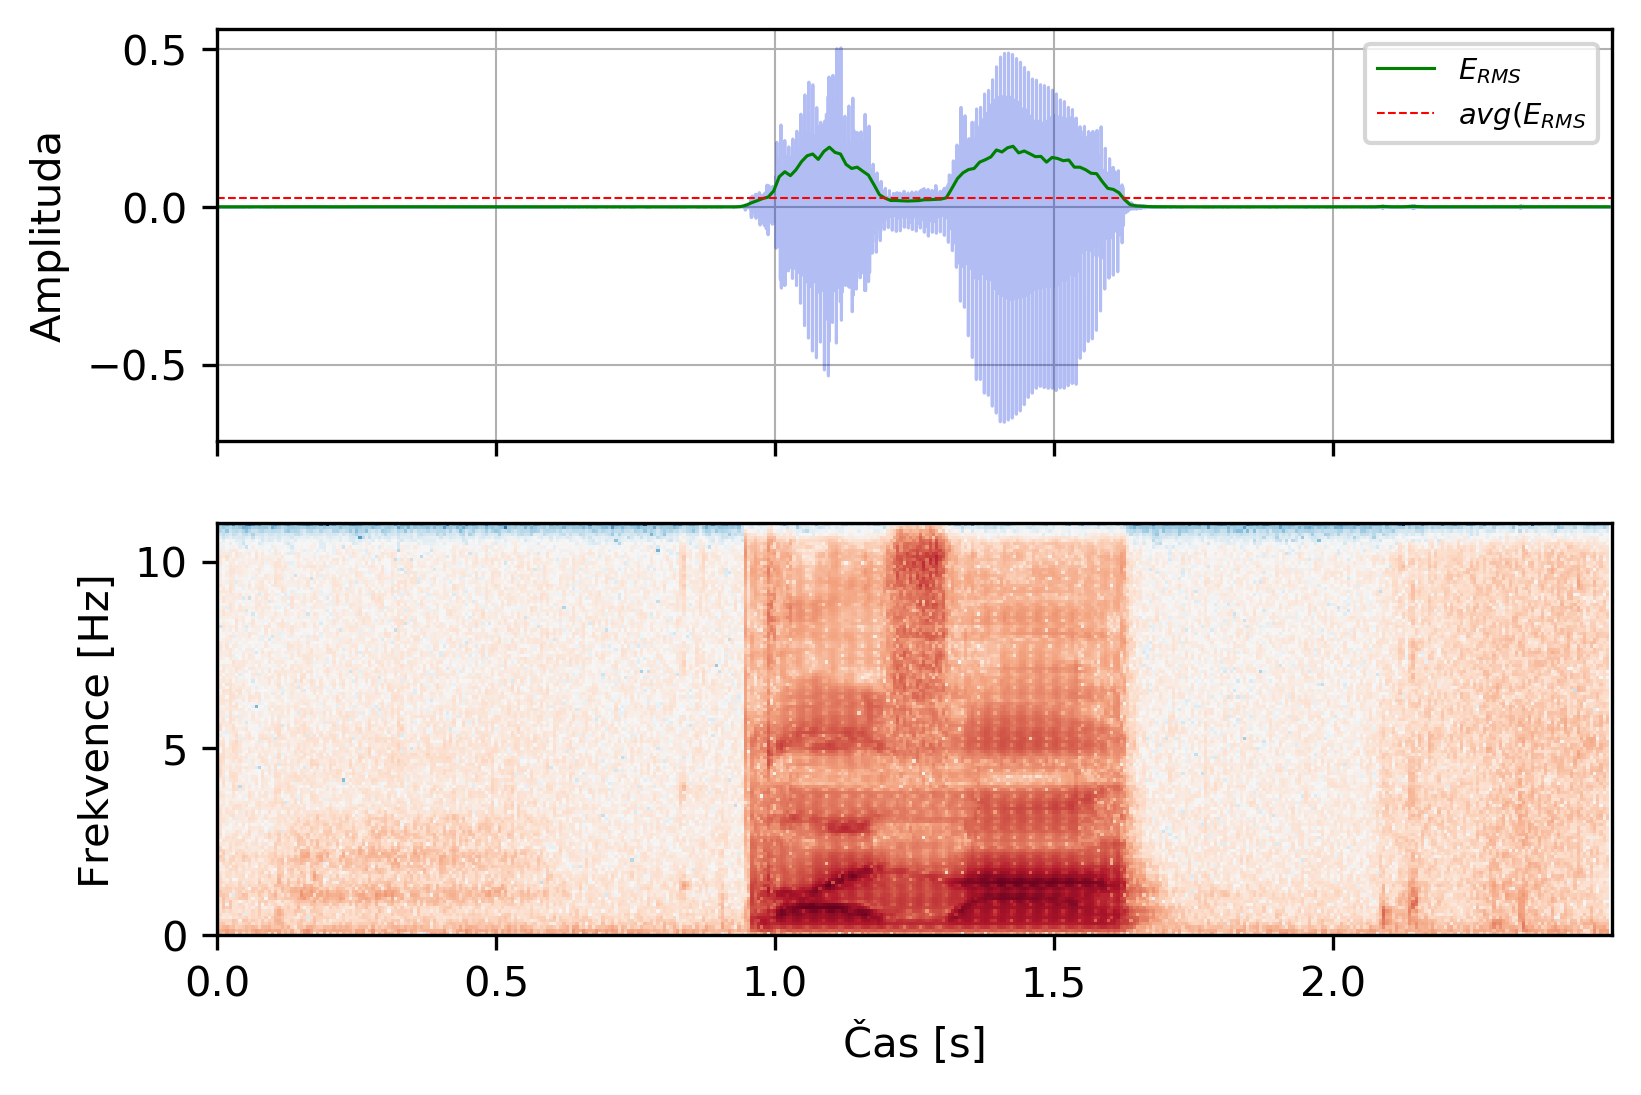
\includegraphics[width=0.9\textwidth]{./ch4-experiments/img/energy_spec_word.png}
  \caption{Průběh a spektrogram slova \uv{kosa} s společně s vyznačenou energií EL promluvy.}
  \label{fig:experiments:normalization:word}
\end{figure}

\begin{figure}[hbpt]
  \centering
  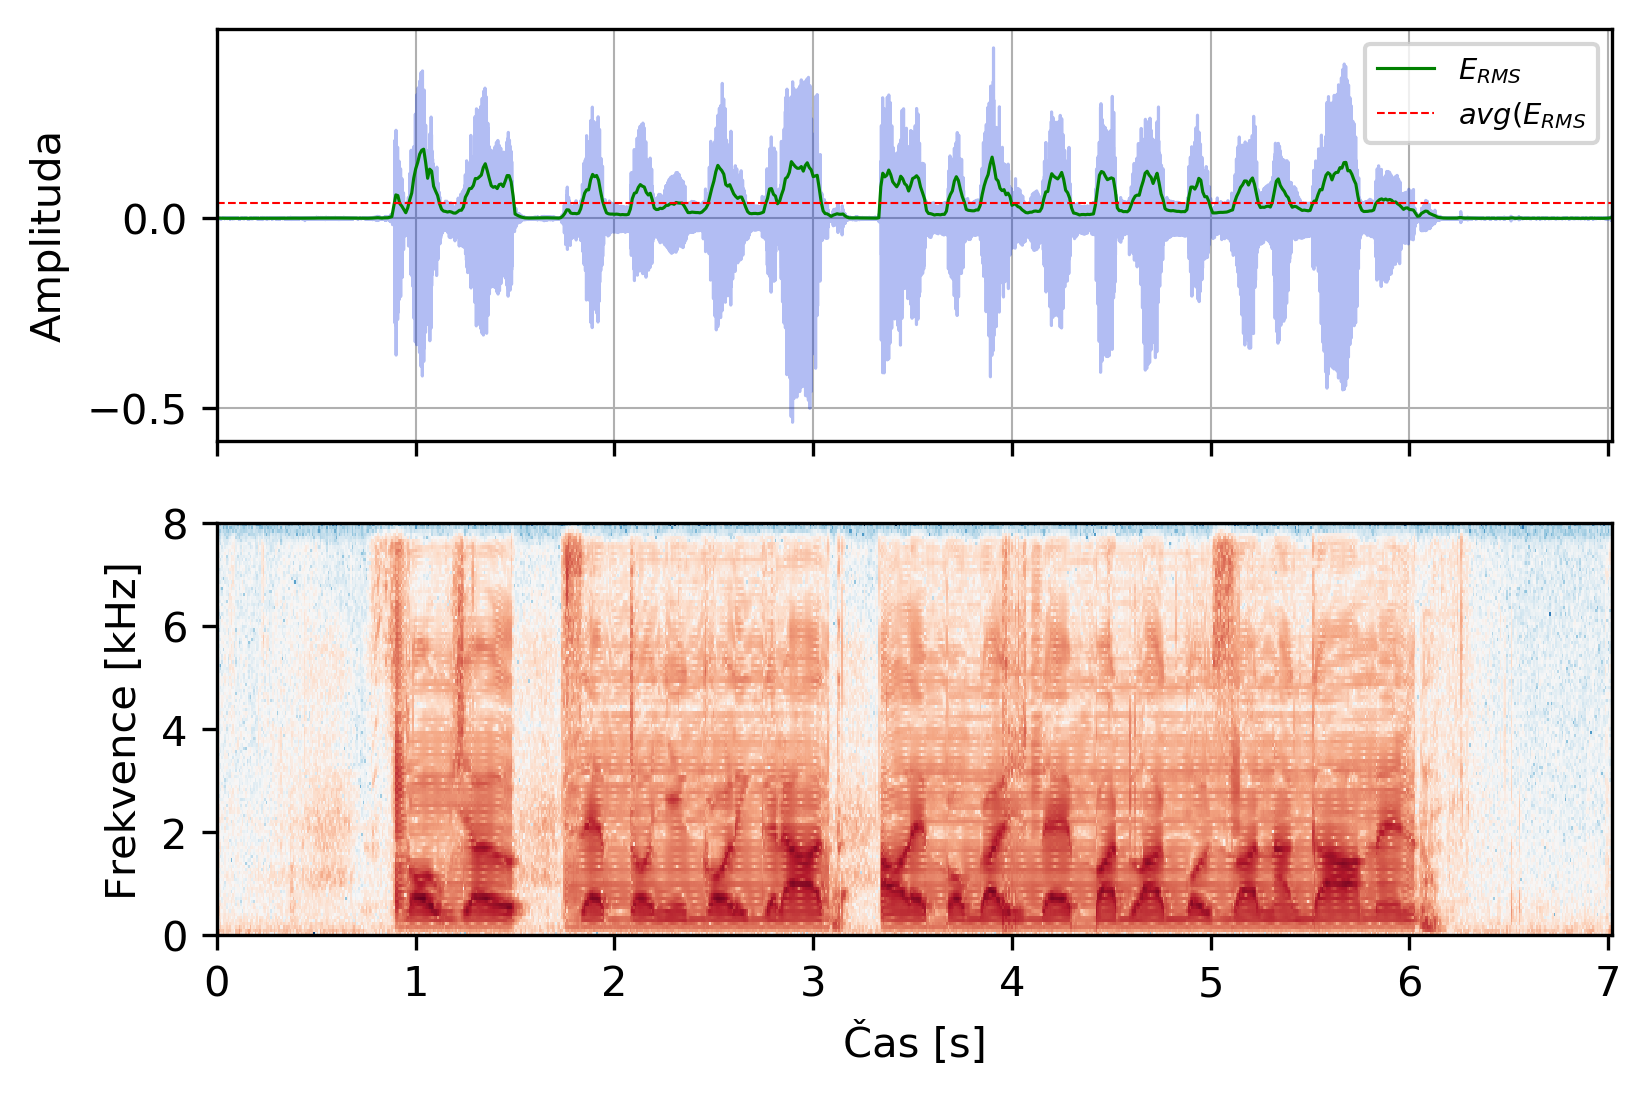
\includegraphics[width=0.9\textwidth]{./ch4-experiments/img/energy_spec_sentence.png}
  \caption{Průběh a spektrogram promluvy obsahující slovo \uv{kosa} a vyznačenou energií EL promluvy.}
  \label{fig:experiments:normalization:sentence}
\end{figure}

Tab. \ref{tab:experiments:normalization:recording} přibližuje souhrnné parametry nahrávek pořízených v 2. etapě nahrávání. Celkem se pořídilo přibližně 2 hodiny řeči (každá nahrávka obsahuje $0,5\ s$ ticha na začátku a konci). Z toho přibližně jen $10\ \%$ představují slova. Společně s novými daty tak korpus obsahuje téměř $14$ hodin audio záznamů.

\begin{table}[htpb]
  \centering
  \def\arraystretch{1.5}
  \pgfplotstabletypeset[
    col sep=comma,
    string type,
    columns/phase/.style={column name=Nahrávání, column type={|l}},
    columns/length/.style={column name=Délka \textit{[HH:MM:SS]}, column type={|r}},
    columns/words/.style={column name=Počet slov, column type={|r}},
    columns/sentences/.style={column name=Počet vět, column type={|r}},
    columns/files/.style={column name=Počet souborů, column type={|r|}},
    every head row/.style={after row=\hline, before row=\hline},
    every last row/.style={after row=\hline},
  ]{./ch4-experiments/tabs/0201-recording-stats.csv}
  \caption{Informace o korpusu nahrávek z 2. etapy nahravání.}
  \label{tab:experiments:normalization:recording}
\end{table}

\subsection{Vliv nových dat na kvalitě modelů}
\label{chap:experiments:normalization:corpus}

Mezi lety 2012 a 2016 zaznamenalo rozpoznávání řeči překotný vývoj používaných technologií. Do té doby byly state-of-the-art modely postaveny na kombinaci HMM a \uv{gaussovských směsí} GMM. U těchto modelů má každý HMM stav jinou směs, viz obr. \ref{fig:experiments:normalization:hmm:gmm}. Pravděpodobnost přechodu mezi stavy HMM pak určují tyto směsi. Jejich parametry jsou získány na základě trénování. S příchodem open source frameworku Kaldi \cite{Kaldi2011} a rozmachem GPU výpočtů se začaly objevovat modely využívající hluboké neuronové sítě (DNN).

Rozpoznávání řeči je možné si představit jako převod jedné sekvence (akustických parametrů) do jiné sekvence (znaků). Pro tento typ úloh se a priory hodí rekurentní neuronové sítě (RNN), ale jejich slabinou je enormní výpočetní náročnost i mimo trénovací fázi a také potřeba enormního množství dat pokud má být vytvořen end-to-end\footnote{End-to-end systémem je ve většině případů myšlen systém, do kterého vstupuje audio (audio příznaky) a vystupuje z něj sekvence znaků.} systém \cite{Hannun2014}. Vytvoření čistě RNN end-to-end ASR systému je nesmírně nákladné (data, HW, atd.), tak se v současné době převážně využívá kombinace HMM modelu, který je také zástupcem rodiny sequence-to-sequence modelů, a DNN. Hlavním rozdílem oproti modelům s GMM je v tom, že pro všechny stavy HMM se trénuje pouze jedna neuronová síť, pomocí které jsou určovány přechody mezi stavy, viz obr. \ref{fig:experiments:normalization:hmm:dnn}. Navíc tím, že tato neuronová síť určuje \uv{pouze} přechody mezi jednitlivými stavy HMM, tak může být tato síť řádově menší a jednodušší, než kdyby se jednalo o end-to-end neuronovou síť.


\begin{figure}[htpb]
  \centering
  \begin{subfigure}[b]{0.4\textwidth}
    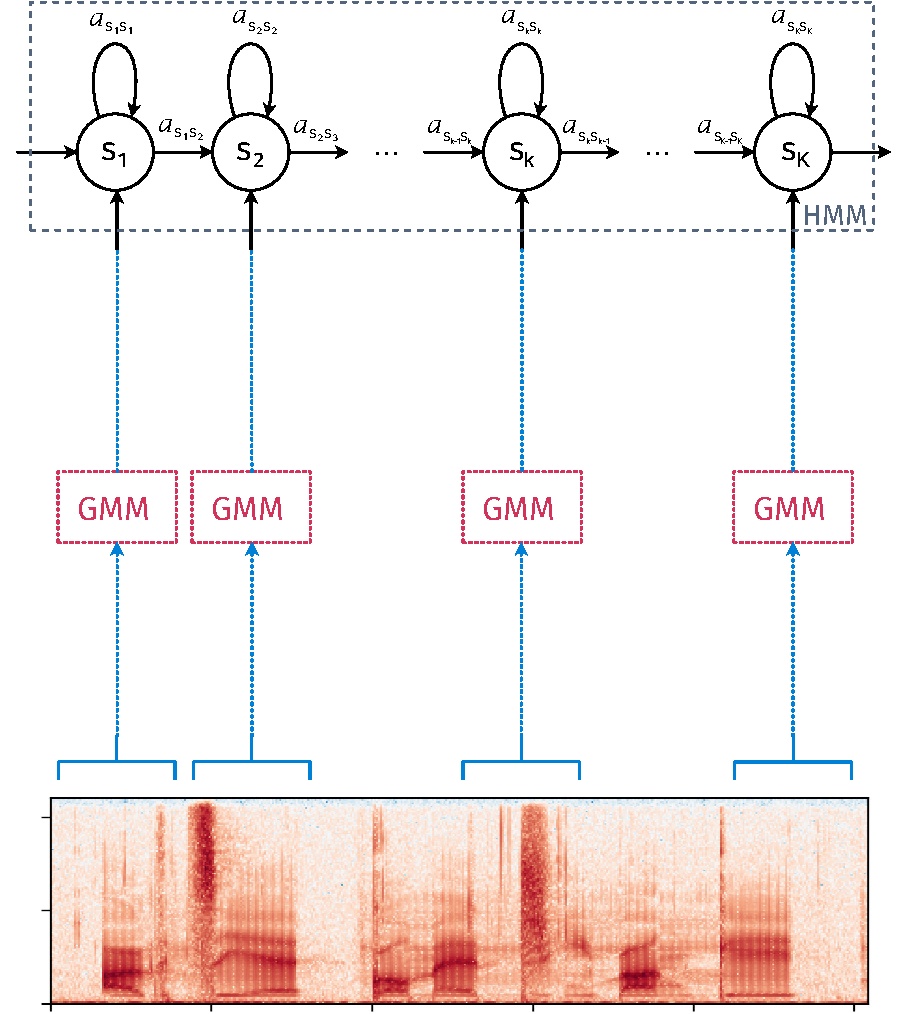
\includegraphics[width=\textwidth]{./ch4-experiments/img/gmm-hmm.pdf}
    \caption{GMM-HMM}
    \label{fig:experiments:normalization:hmm:gmm}
  \end{subfigure}
  %
  \begin{subfigure}[b]{0.4\textwidth}
    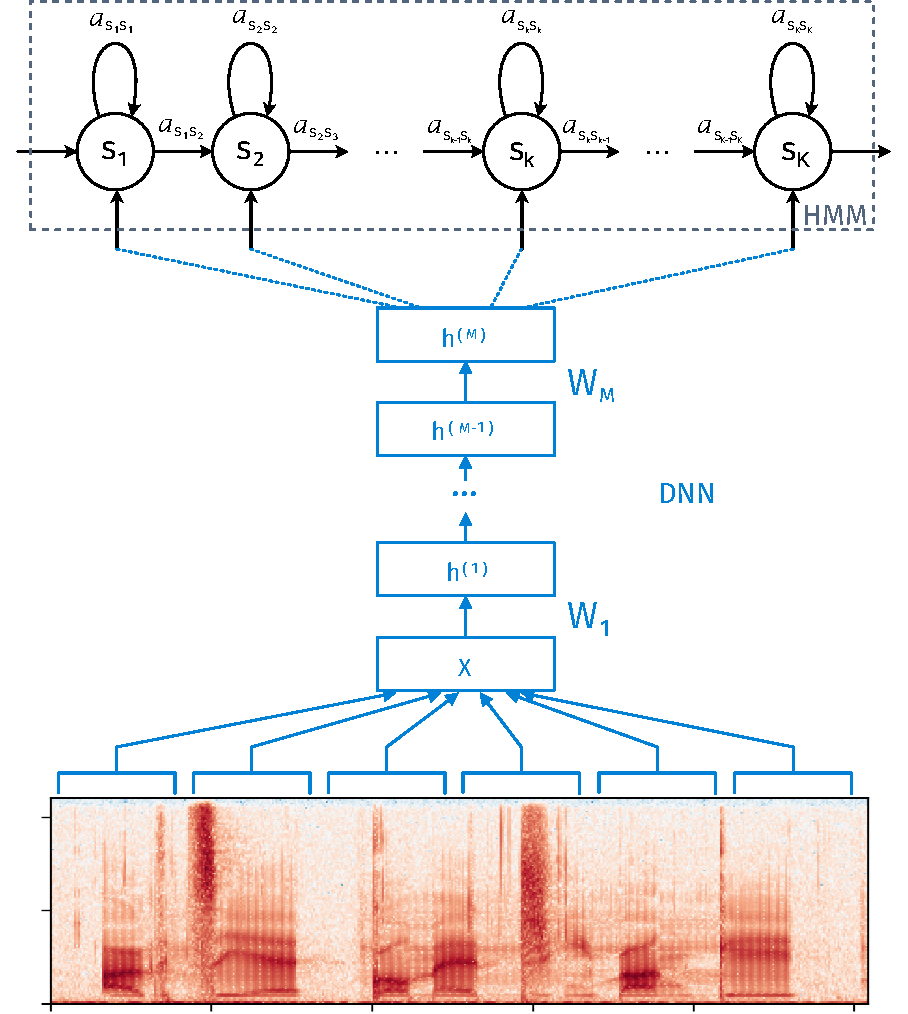
\includegraphics[width=\textwidth]{./ch4-experiments/img/dnn-hmm.pdf}
    \caption{DNN-HMM}
    \label{fig:experiments:normalization:hmm:dnn}
  \end{subfigure}
  \caption{Znázornění odlišného principu \textit{GMM-HMM} a \textit{DNN-HMM}.}
  \label{fig:experiments:normalization:hmm}
\end{figure}

S novými daty je možné natrénovat modely a ověřit, zda je s nimi systém schopen pracovat. Oproti \ref{chap:experiments:analysis:experiment} je použit framework Kaldi, který se stal standardem pro vytváření akustikých modelů. Samotný framework se skládá z velkého množství utilit, která každá plní určitý \uv{jednoduchý} úkol v procesu vytváření modelu. Kompletní proces vytváření modelu se tak sestává v postupném spouštění těchto utilit v přesně definovaném pořadí. Autoři frameworku připravili nepřeberné množství skriptů, které slouží k vytvoření různých modelů. Všechny modely pro EL řeč vycházejí ze skriptů pro natrénování modelů z Wall Street Journal (WSJ) korpusu, který nejčastěji jako jakýsi benchmark ASR systémů. Skripty jsou jen drobně upraveny, aby výsledný model odpovídal EL doméně a bylo jej vůbec možné vytvořit.

Přestože DNN nahradily GMM v HMM, tak k jejich natrénování je nezbytné nejprve natrénovat \textit{GMM-HMM} model, který slouží k prvotnímu zarovnání (určení hranic jednotlivých fonémů v rámci audio náhrávky). Toto zarovnání slouží jako startovní bod pro neuronovou síť. Tím, že je trénována pouze jedna síť, tak je k dispozici řádově více dat\footnote{V případě \textit{GMM-HMM} má každý stav své GMM a tím pádem, čím více stavů, tím méně trénovacích dat pro každou směs.} k jejímu natrénování, na druhou stranu má tato síť mnohem více parametrů než všechny GMM směsi dohromady a tak je potřeba dbát na velikost sítě. Nicméně pro standardní WSJ DNN (6 vrstev, každá s 2048 nebo 4096 neurony) je dat dostatek.

Přestože vývoj výpočetních GPU postupuje závratnou rychlostí, tak natrénování standardního \textit{DNN-HMM} modelu trvá o poznání déle než \textit{GMM-HMM}. Pro ověření zda je možné vytvořit model ze všech dat, která jsou k dispozici poslouží i \textit{GMM-HMM} model, protože ten slouží jako startovní bod pro \textit{DNN-HMM}. Pokud tyto modely neposkytnou DNN, alespoň trochu \uv{dobré} počáteční podmínky, tak sofistikovanější DNN nemusí pomoci.

Pro potřeby ověřovacího experimentu posloužily jako základ Kaldi WSJ skripty. Jako první je vytvořen monofónový akustický model používající Perceptual Linear Prediction (PLP) s 12 kepstrálními, delta a delta-delta koeficienty. Tento monofónový model je speciální případ kontextově závislých modelů, bez levého a pravého (fonémového) kontextu. Následně jsou natrénovány trifónové modely. Stejně jako v experimentech provedených v části \ref{chap:experiments:analysis:experiment}, tak i zde jsou použity rozhodovací stromy, protože počet všech variant trifónů je příliš velký.

V části \ref{chap:experiments:analysis:experiment} byl korpus rozdělen na trénovací a testovací sadu. Po rozšíření korpusu bylo rozdělení dat z 1. etapy ponecháno a nová data rozdělena mezi trénovací a testovací sadu. Všechny nahrané věty v 2. etapě jsou použity v trénovací a všechna slova naopak v testovací sadě. Toto rozdělení je logické, protože důvodem rozšíření korpusu byla snaha ověřit funkčnost ASR systémů na slovech, která mají odlišný význam, ale liší se pouze znělostí jednoho fonému. Jelikož z výsledku v části \ref{chap:experiments:analysis:reduction} vyplývá, že určité spektrum trifónů je možné reprezentovat pouze pomocí znělých variant, tak při použití nahraných slov bude teoreticky možné lépe prozkoumat tuto otázku.

Po otestování výše popsaného modelu byl opět použit monofónový zerogramový jazykový model tak, aby co nejméně ovlivňoval dosažené výsledky. Na kompletní testovací sadě bylo dosaženo přesnosti $54,96\ \%$ a v případě, že testovací sada obsahovala pouze nově nahraná slova, tak dokonce jen $42,97\ \%$. Což je významné zhoršení oproti výsledkům dosažených v \ref{chap:experiments:analysis:experiment}, kde bylo dosaženo více něž $80\ \%$ přesnosti.

Pro ověření, že není chyba v procesu trénování (přeci jen se změnil framework) poslouží křížový test, kdy pomocí stejného procesu jsou natrénovány modely z původních (1. etapa) a nových (2. etapa) dat a křížově otestovány na kompletní, původní a jen nové části testovací sady. Výsledky tohoto testu jsou v tab. \ref{tab:experiments:normalization:cross}. Z tabulky je jasně patrné, že pokud je model natrénován a otestován pomocí dat ze stejné etapy, tak je dosaženo podobných výsledků jako v \ref{chap:experiments:analysis:experiment}.

%model;orig;new

\begin{table}[htpb]
  \centering
  \def\arraystretch{1.5}
  \pgfplotstabletypeset[
    col sep=semicolon,
    string type,
    columns/model/.style={column name=Model, column type={|c}},
    columns/orig/.style={column name=1. etata $[\%]$, column type={|r}},
    columns/new/.style={column name=2. etapa $[\%]$, column type={|r|}},
    every head row/.style={before row={
      \hline
      & \multicolumn{2}{c|}{Accuracy} \\
    },after row=\hline},
    every last row/.style={after row=\hline},
  ]{./ch4-experiments/tabs/0202-cross_test.csv}
  \caption{Křížový test modelů natrénovaných a otestovaných na datech z 1. a 2. etapy.}
  \label{tab:experiments:normalization:cross}
\end{table}

% - 20161208_param -> porovnani n vs o, vzit hodnoty z toho
% - 20170111_together -> CMN FULL vysledky na HMM, pak tam dat i vysledky z

Z dosažených výsledků tedy vyplývá, že nová data jsou příliš odlišná od původních dat a v parametrickém prostoru příliš vzdálena těm původním. Zároveň je těchto dat relativně malé množství, aby se mohly modely plně adaptovat. Na rozdíl v datech se můžeme koukat jako na změnu kanálu, která je příčinou těchto změn, protože řečník je stejný. V předchozím textu bylo zmíněno, že v rámci 2. etapy došlo ke změné nahrávací procedury a také elektrolarynxu. Tím byl pozměněn kanál a logicky výsledná zaznamenaná řeč má jiné parametry než ta v 1. etapě. Mezi další prvky, které mohou způsobit změnu kanálu může být prostředí, tedy jestli je řeč produkována uvnitř nějaké místnosti, či venku, jestli je na pozadí přítomen šum atd. K tomu, aby bylo možné použít všechna dostupná data, je potřeba eliminovat tento vliv kanálu. K jeho eliminaci je možné využít CMN, což je zkratka anglických slov Cepstral Mean Normalisation. Principem této metody je odstranení vlivu kanálu na základě střední hodnoty kepstrálních koeficientů, viz dále.

Zaznamenaný signál je možné popsat jako

\begin{equation}
  y\left[n\right] = x\left[n\right] \circledast h\left[n\right],
  \label{eq:experiments:normalization:convolution}
\end{equation}

\noindent kde $x\left[n\right]$ představuje vstupní signál, tedy řeč, a $h\left[n\right]$ odezva kanálu na jednotkový impulz. Zaznamenaný signál je jejich lineární konvolucí. Ve frekvenční oblasti je pak rovnice \ref{eq:experiments:normalization:convolution} zapsaná následovně:

\begin{equation}
  Y\left[f\right] = X\left[f\right] \cdot H\left[f\right]
\end{equation}

\noindent V této oblasti se z konvuluce stalo násobění, což značně zjednodušuje situaci. K odstranění vlivu kanálu je, ale ještě potřeba převést hodnoty do kepstrálná oblasti. To je realizováno pomocí logaritmu spektra

\begin{equation}
  Y\left[q\right] = \log\left(Y\left[f\right]\right) = \log\left(X\left[f\right] \cdot H\left[f\right]\right) = X\left[q\right] + H\left[q\right],
\end{equation}

\noindent kde $q$ představuje kepstrální koeficient. V kepstrální oblasti je vliv kanálu aditivní složkou výsledného záznamu. Problémem však je, že konkrétní hodnota vlivu kanálu je neznáma, protože k dispozici je pouze výsledný ovlivněný signál. Předpokládejme však, že vliv kanálu je stacionární\footnote{Jedná se sice o silný, ale logický předpoklad. Pokud se vztáhne k pořízenému řečovému korpusu, tak v rámci jedné etapy nahrávání, je proces nahrávání neměnný, tzn. je použita stejná aparatura a k nahrávání dochází vždy ve stejné místnosti.}, tak poté je možné každý frame nahrávky $i$ zapsat jako

\begin{equation}
  Y_i\left[q\right] = H\left[q\right] + X_i\left[q\right],
\end{equation}

\noindent kde $Y_i\left[q\right]$ představuje $i$ frame kepstra $q$ nahrávky a $X_i\left[q\right]$ představuje $i$ frame kepstra $q$ neovlivněné řeči. Z této rovnice je pak možné vypočítat střední hodnotu

\begin{equation}
  \frac{1}{N} \sum_i Y_i\left[q\right] = H\left[q\right] + \frac{1}{N} \sum_i X_i\left[q\right].
\end{equation}

\noindent Vliv kanálu je pak možné eliminovat odečtením střední hodnoty kepstra $q$ od aktuální hodnoty kepstra $Y_i\left[q\right]$

\begin{align}
  R_i\left[q\right] &= Y_i\left[q\right] - \dfrac{1}{N}\sum_{j} Y_j\left[q\right] \nonumber  \\
  &= H\left[q\right] + X_i\left[q\right] - \left( H\left[q\right] + \frac{1}{N} \sum_j X_j\left[q\right] \right) \nonumber  \\
  &= X_i\left[q\right] - \frac{1}{N} \sum_j X_j\left[q\right]
  \label{eq:experiments:normalization:cmn}
\end{align}

\noindent S pomocí rovnice \ref{eq:experiments:normalization:cmn} je možné odfiltrovat vliv kanálu a teoreticky tak získat hodnoty kepstrálních koeficientů odpovídající nezkreslené řeči. Otázkou je přes jaký úsek počítat střední hodnotu. Je možné ji počítat přes posuvné okénko fixní délky, přes jednotlivé nahrávky, nebo dokonce přes všechny nahrávky konkrétní etapy. Pokud totiž bude úsek, přes který je počítána průměrná hodnota krátký, tak se může stát, že vypočtená střední hodnota nebude odpovídat skutečné střední hodnotě umožňující eliminaci vlivu kanálu. V tomto případě, kdy nahrávky dělí velký časový úsek a i proces nahrávání byl změněn, je toto potřeba odexperimentovat.

\subsection{Poslechový test}

\subsection{Výsledky porovnání}

\begin{itemize}
  \item popsat důvody proč potřebujeme další nahrávky (slova, která se liší znělostí)
  \item popsat algoritmus výberu slov/vět k nahrávání
  \item napsat něco o tom, že mezi nahráváními byl velký časový rozestup a taky se změnila technika nahráváními
  \item problém taky s tím, že první sada nahrávek je mnohem větší (10h) než ta nová (cca 30 min) a modely tak nefungovali na nových datech v testovací sade
  \item použití neuronovek (Kaldi)
  \item popis a výsledky experimentu \uv{člověk vs. stroj}
\end{itemize}
